\title{Concurrency and Parallel Programming \\ Assignment 2}
\author{David van Erkelens and Jelte Fennema \\ Department of Computer Science
    \\ University of Amsterdam} \date{\today}
\documentclass[12pt]{article}
\usepackage{graphicx}
\usepackage{color}
\begin{document}
\maketitle
\section{Notes}
\begin{itemize}

\item The smallest problem size doesn't benefit from MPI in any of the cases. This was also the case with threading.

\item For some reason the tests with problem size $10^5$ performed abnormaly bad in all of the tests . It only benefits a bit from MPI. Way less than any of the others. (except for $10^3$) Both $10^4$ and $10^6$ perform way better in all cases.

\item With the two largest problem sizes MPI gains around the maximum theoritical speedup when running on two different nodes with one process per node. In comparisson with using threading MPI performs very well in these cases.

\item
As seen in the graphs, the speedup depends on the problem size. When the problem size is small, the speedup is also very small and sometimes even smaller that 1. With a large problem size, the speedup can reach almost 8. This can be explained by the fact that there can be a large communication delay with a small problem size. However, when there is a larger problem size (and thus more calculations), the communication delay will be a smaller percentage of the total executing time.
\item
As seen in the graphs, all problem sizes quickly reach their maximum possible speedup. Only the larges problem size doesn't stagnate yet. However, when the problem will be executed on even more cores, this problem size will probably also stagnate, but there's no way to retreive this from the current results.


\end{itemize}
\section{Graphs}
\includegraphics[width=\textwidth]{onenode.jpg}
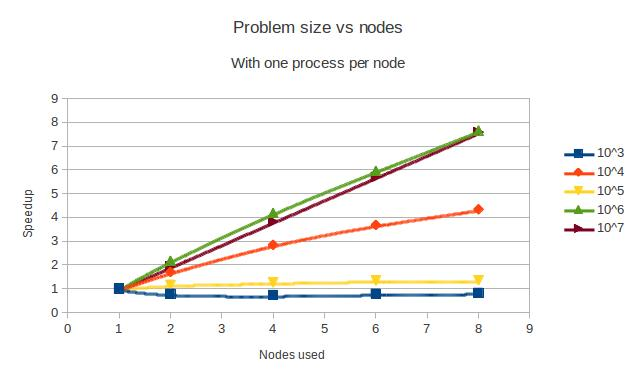
\includegraphics[width=\textwidth]{oneproc.jpg}
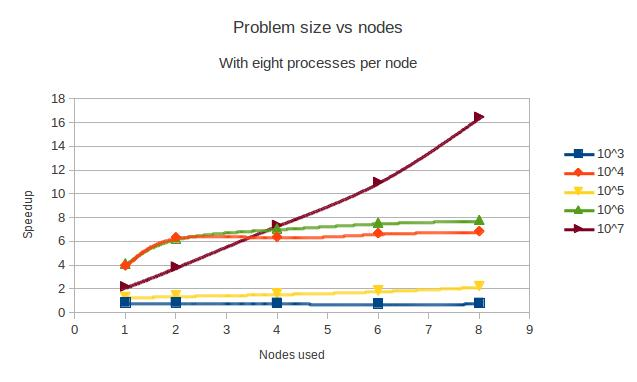
\includegraphics[width=\textwidth]{eightproc.jpg}
\end {document}
